\documentclass[10pt,a4paper,ragged2e,withhyper]{altacv}

% -----------------------
% PACKAGES
% -----------------------
\usepackage[utf8]{inputenc}
\usepackage[T1]{fontenc}
\usepackage{paracol} % Needed for two-column layout
\usepackage{graphicx}
\usepackage{svg}
\svgpath{{icons/}}
\usepackage{fontawesome5}
\usepackage{hyperref}
\usepackage{pgfplots}
\usepackage{tikz}
\usepackage{enumitem}
\usepackage{xcolor}
\usepackage{geometry}

% -----------------------
% MODERN DEVELOPER FONTS
% -----------------------
% Use monospace font for developer aesthetic
\usepackage{lmodern}
\renewcommand{\familydefault}{\ttdefault} % Use typewriter font
\usepackage[scaled=0.85]{beramono} % Modern monospace font

% -----------------------
% DOCKER-INSPIRED COLOR PALETTE
% -----------------------
\definecolor{DockerBlue}{HTML}{2496ED}      % Docker Primary Blue
\definecolor{DockerDark}{HTML}{24292F}      % GitHub Dark
\definecolor{DockerLight}{HTML}{F6F8FA}     % GitHub Light Background
\definecolor{DockerGray}{HTML}{6A737D}      % GitHub Gray Text
\definecolor{DockerSuccess}{HTML}{28A745}   % Success Green
\definecolor{DockerWarning}{HTML}{FFC107}   % Warning Yellow
\definecolor{DockerDanger}{HTML}{DC3545}    % Error Red
\definecolor{DockerPurple}{HTML}{6F42C1}    % Purple accent
\definecolor{DockerBorder}{HTML}{E1E4E8}    % Light border

% Modern color assignments
\colorlet{heading}{DockerBlue}
\colorlet{accent}{DockerBlue}
\colorlet{emphasis}{DockerDark}
\colorlet{body}{DockerGray}
\colorlet{lightbg}{DockerLight}
\colorlet{border}{DockerBorder}

% -----------------------
% MODERN 2024 LAYOUT
% -----------------------
\geometry{margin=1cm} % 1cm margins as requested
\usetikzlibrary{positioning,shapes.geometric,arrows.meta,shadows,decorations.pathreplacing}
\usepackage{tcolorbox}
\tcbuselibrary{skins}
\usepackage{tikz}

% Card with tiny light border, rounded corners
\tcbset{
  vercelcard/.style={
    enhanced,
    boxrule=0.4pt,
    colback=white,
    colframe=DockerBorder,
    arc=6pt,
    outer arc=6pt,
    top=14pt,
    bottom=14pt,
    left=18pt,
    right=18pt,
    boxsep=0pt
  }
}

% Timeline card with light border
\tcbset{
  timelinecard/.style={
    enhanced,
    boxrule=0.5pt,
    colback=white,
    colframe=DockerBorder,
    arc=6pt,
    top=12pt,
    bottom=12pt,
    left=16pt,
    right=16pt
  }
}

% Modern skill icon with SVG support (SVG files in icons/)
\newcommand{\skillicon}[2]{%
  \tikz[baseline=(icon.base)]{
    \node[circle, fill=#1!8, draw=#1!20, minimum size=22pt, inner sep=1pt] (icon) {\includesvg[width=12pt,height=12pt]{#2}};
  }%
}

% Fallback text icon for missing SVGs
\newcommand{\textskillicon}[2]{%
  \tikz[baseline=(icon.base)]{
    \node[circle, fill=#1!8, draw=#1!20, minimum size=22pt, font=\tiny\ttfamily] (icon) {#2};
  }%
}

% Timeline node command
\newcommand{\timelinenode}[1]{%
  \tikz[baseline=(node.base)]{
    \node[circle, fill=#1, minimum size=12pt, inner sep=0pt] (node) {};
  }%
}

% Horizontal percentage skill bar
\newcommand{\skillbar}[2]\par\vspace{2pt}%
  \begin{tikzpicture}[x=\linewidth,y=1cm]
    \fill[DockerBorder] (0,0) rectangle (1,0.12);
    \pgfmathsetmacro{\p}{#2/100}
    \fill[DockerBlue] (0,0) rectangle (\p,0.12);
  \end{tikzpicture}\vspace{4pt}
}

% Project item macro (uniform format)
\newcommand{\projectitem}[6]{%
  \textbf{#1}\\
  \textcolor{body}{#2}\\[4pt]
  \cvtag{\faGithub\ #3}\\[2pt]
  \textcolor{DockerGray}{\small #4}\\
  \textcolor{DockerGray}{\small #5\ on\ \faCodeBranch\ #6}
}

% -----------------------
% PERSONAL INFO
% -----------------------
\name{Marcos Example}
\tagline{Software Engineer • Full Stack Developer}
\photoL{3cm}{photo.png} % ← Add your photo.png in same folder or comment this line

\personalinfo{
  \email{marcos@example.com}
  \phone{+1 234 567 890}
  \github{marcosdev}
  \linkedin{marcos-dev}
  \homepage{marcos.dev}
}

% -----------------------
% DOCUMENT BODY
% -----------------------
\begin{document}

% Full-width gradient header, margin-top 0 (overlay), vertically centered content
\noindent
\begin{tikzpicture}[remember picture,overlay]
  % background gradient spanning full paper width
  \fill[left color=DockerBlue!85, right color=DockerPurple!70]
    (current page.north west) rectangle ([yshift=-4.3cm]current page.north east);
  % content container centered vertically within header height
  \node[anchor=north west, inner sep=0pt] at (current page.north west) {
    \begin{minipage}[c][4.3cm][c]{\paperwidth}
      \hspace*{1cm}% left padding to align roughly with text area
      \begin{minipage}[c]{0.22\paperwidth}
        \centering
% Circular photo using overzoom to center image within circle
\tikz{\path[fill overzoom image={photo.png}] circle[radius=1.5cm];}
      \end{minipage}\hfill
      \begin{minipage}[c]{0.72\paperwidth}
        {\color{white}{\Huge\bfseries Marcos Example}}\\[6pt]
        {\color{white!90}{\Large Software Engineer \& Full Stack Developer}}\\[6pt]
        {\color{white!85}{marcos@example.com \quad +1\;234\;567\;890 \quad github.com/marcosdev}}
      \end{minipage}
    \end{minipage}
  };
\end{tikzpicture}
% Reserve space below the overlay header (optimize vertical space)
\vspace*{3.9cm}

% About section spans full width
\begin{tcolorbox}[vercelcard]
\textcolor{DockerBlue}{\large\textbf{About}}

\vspace{8pt}

I'm a \textbf{passionate software engineer} with deep expertise in crafting elegant solutions to complex problems. My journey spans from building interactive data visualizations to architecting scalable systems.

\vspace{6pt}

Currently focused on \textcolor{DockerBlue}{\textbf{AI/ML engineering}} and modern web technologies, with a passion for clean architecture and developer experience.

\end{tcolorbox}

\vspace{16pt}

% Two-column layout for the rest
\columnratio{0.58}
\begin{paracol}{2}

% LEFT COLUMN -----------------------
\begin{tcolorbox}[vercelcard, sidebyside, righthand width=0.42\linewidth, sidebyside gap=16pt]
\textcolor{DockerBlue}{\large\textbf{Capabilities}}\\[6pt]

% LEFT: Technologies (icons)
\textcolor{emphasis}{\textbf{Technologies}} \\
\vspace{4pt}
\textbf{Frontend}\\
\skillicon{DockerBlue}{react-original} \hspace{4pt}
\skillicon{DockerSuccess}{typescript-original} \hspace{4pt}
\skillicon{DockerWarning}{javascript-original}\\[8pt]
\textbf{Backend}\\
\skillicon{DockerWarning}{python-original} \hspace{4pt}
\skillicon{DockerPurple}{postgresql-original}\\[8pt]
\textbf{AI / ML}\\
\skillicon{DockerDanger}{tensorflow-original} \hspace{4pt}
\skillicon{DockerPurple}{pytorch-original}\\[8pt]
\textbf{DevOps \& Tools}\\
\skillicon{DockerBlue}{docker-original} \hspace{4pt}
\skillicon{emphasis}{linux-original} \hspace{4pt}
\skillicon{DockerGray}{github-original}

\tcblower
% RIGHT: Skills radar
\begin{center}
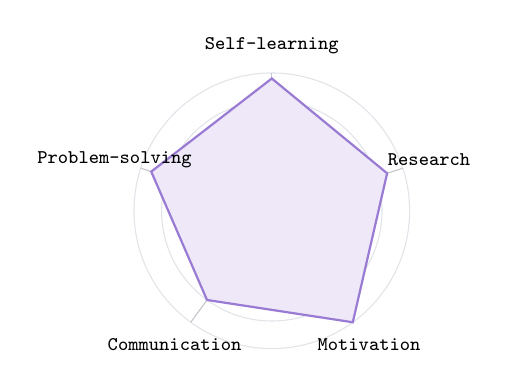
\begin{tikzpicture}[scale=0.7]
  \foreach \r in {1,2,3,4,5} {\draw[DockerBorder, thin] (0,0) circle (\r*0.5cm);}  
  % axes (Self-learning, Research, Motivation, Communication, Problem-solving)
  \draw[DockerGray!40] (0,0) -- (90:2.5cm);
  \draw[DockerGray!40] (0,0) -- (18:2.5cm);
  \draw[DockerGray!40] (0,0) -- (-54:2.5cm);
  \draw[DockerGray!40] (0,0) -- (-126:2.5cm);
  \draw[DockerGray!40] (0,0) -- (162:2.5cm);
  % data polygon (example levels)
  \draw[DockerPurple!70, fill=DockerPurple!12, thick]
    (90:2.4cm) -- (18:2.2cm) -- (-54:2.5cm) -- (-126:2.0cm) -- (162:2.3cm) -- cycle;
  \node[font=\scriptsize] at (90:3.0cm) {Self-learning};
  \node[font=\scriptsize] at (18:3.0cm) {Research};
  \node[font=\scriptsize] at (-54:3.0cm) {Motivation};
  \node[font=\scriptsize] at (-126:3.0cm) {Communication};
  \node[font=\scriptsize] at (162:3.0cm) {Problem-solving};
\end{tikzpicture}
\end{center}
\end{tcolorbox}


\vspace{12pt}

\begin{tcolorbox}[vercelcard]
\textcolor{DockerBlue}{\large\textbf{Education}}

\vspace{8pt}

\textbf{B.Sc. Computer Science} \\
\textcolor{body}{University of Example} \\
\textcolor{DockerGray}{\small 2018 -- 2022}

\end{tcolorbox}

\vspace{12pt}

\begin{tcolorbox}[vercelcard]
\textcolor{DockerBlue}{\large\textbf{Projects}}

\vspace{8pt}

% Project 1
\projectitem{DataVizPro}{Interactive data visualization platform}{Marcos/repo-datavizpro}{Initial release}{Oct 10}{main}\\[6pt]
\skillicon{DockerBlue}{react-original} \hspace{3pt}
\skillicon{DockerWarning}{javascript-original} \hspace{3pt}
\skillicon{DockerSuccess}{python-original}\\[10pt]

% Project 2
\projectitem{portfolio}{marcos.oriol-tech.com}{MarcosOriolPago/portfolio}{feat: changed profile photo}{Oct 14}{main}\\[6pt]
\skillicon{DockerBlue}{react-original} \hspace{3pt}
\skillicon{DockerGray}{github-original}

\end{tcolorbox}



% RIGHT COLUMN -----------------------
\switchcolumn

\begin{tcolorbox}[vercelcard]
\textcolor{DockerBlue}{\large\textbf{Career History}}

\vspace{8pt}

% Vertical timeline with dots on the left, constrained to column width
\begin{tikzpicture}[x=1cm,y=1cm]
  % vertical line within box (extended for added spacing)
  \draw[DockerBorder, line width=0.8pt] (0,0) -- (0,-12.2);

  % Entry 1 (top)
  \fill[DockerPurple] (0,0) circle (3pt);
  % Title aligned with dot
  \node[anchor=west] at (0.45,0) {\textcolor{DockerPurple}{\bfseries AI - ML Engineer}};
  % Company
  \node[anchor=west,text=emphasis] at (0.45,-0.50) {IDNEO Technologies Inc.};
  % Place
  \node[anchor=west,text=body] at (0.45,-1.00) {\small Barcelona, Spain};
  % Years
  \node[anchor=west,text=DockerGray] at (0.45,-1.50) {\small 2024 -- present};
  % Description (wrapped)
  \node[anchor=west,align=left,text width=\dimexpr\linewidth-1.3cm\relax] at (0.45,-2.30) {Development of AI Models for embedded systems in the automotive industry, including data collection, model training, and deployment.};
  % Icons
  \node[anchor=west] at (0.45,-3.10) {\skillicon{DockerWarning}{python-original}\hspace{3pt}\skillicon{DockerBlue}{docker-original}\hspace{3pt}\skillicon{DockerDanger}{tensorflow-original}\hspace{3pt}\skillicon{DockerPurple}{pytorch-original}};

  % Entry 2 base y (extra gap)
  \def\ybase{-7.6}
  \fill[DockerBlue] (0,\ybase) circle (3pt);
  % Title
  \node[anchor=west] at (0.45,\ybase) {\textcolor{DockerBlue}{\bfseries Software Engineer}};
  % Company
  \node[anchor=west,text=emphasis] at (0.45,\ybase-0.50) {PRBB};
  % Place
  \node[anchor=west,text=body] at (0.45,\ybase-1.00) {\small Barcelona, Spain};
  % Years
  \node[anchor=west,text=DockerGray] at (0.45,\ybase-1.50) {\small 2024 -- 2025};
  % Description
  \node[anchor=west,align=left,text width=\dimexpr\linewidth-1.3cm\relax] at (0.45,\ybase-2.30) {Developing and implementing artificial intelligence tools for software designed for ultrasonic-based spinal cord stimulation.};
  % Icons
  \node[anchor=west] at (0.45,\ybase-3.10) {\skillicon{DockerSuccess}{react-original}\hspace{3pt}\skillicon{DockerWarning}{python-original}\hspace{3pt}\skillicon{DockerPurple}{postgresql-original}};
\end{tikzpicture}

\end{tcolorbox}


\end{paracol}

\end{document}
